\chapter{Modeling Cyber-Insurance }
\label{chp:modelingCyberInsurance} 


\section{Network Formation}



In many scenarios agents seeks to create networks in order to directly benefit from each other. The established links might represent companies out sourcing part of their manufacturing, or cooperative agreements in the development of new software products. In addition to increase the trade-off, each of the established links represents risk of being a victim of cascading failures. The intuitive example is the spread of epidemic diseases, also  (node failures of a power grid and) financial contagion such as the one back in 2008 was a result of cascading failures. Strategic network formation using cyber-insurance can be used to prevent such situation in addition to increase the overall payoff of participants in a clustered network.


When deciding whether to establish connection to a neighbor agent, the payoff has to be a balance between the expected earnings and the risk of the other party failing to complete the transaction. This is the reason why we seek to only download content from trusted peers and outlaw MC-gangs are consistently skeptical to enter into new agreements despite promising increased earnings, since the risk of undercover police are too high. 


The paper \cite{contagion} describes a model which seeks to capture the underlying trade-off between the benefits of adding new links and the problem with increased contagious risk. Results from the model describes a situation where clustered graphs achieve a higher payoff when connected to trusted agents. This phenomena is called super-critical payoffs. Unlike in anonymous graphs, which are completely random, nodes in these graphs share some information with their neighbors, which is used when deciding whether to connect or not. The cliques, forms a clustered network of agents which trust each other, consequently the risk of cascading failures are lower.
Inspired by this model, we created a model which shields light on how cyber-insurance can be used in network formation to prevent cascading failures and increase an agents payoff.  

\subsection{Model of handling contagion risk}
The model is simplified in order to show the concept of using cyber-insurance to encounter the problems with contagious risk. The model is formulated as follows. A set of $n$ agents are randomly chosen to be insured or not. They all get their own income, and by connecting to other agents they will benefit from their income, i.e. when connected both agents will increase their income. However, when connecting to another agent naturally the cost of insurance increases due to aggregated risk. If and agent connects to someone without insurance a possible risk of severe losses due to cascading failure $r$ has to be taken into account. 

\begin{tabular}{|l|}
  \hline
  $\alpha$ - an agents income\\
  $\beta$ - income from direct links \\
  $I_{o}$ - cost of insurance. \\
  $I_{l}$ - increased insurance cost due to risk from a direct link.\\
  $r$ - cost of not having insurance, in case of failure.\\
  \hline
\end{tabular} \\

Each agents payoff $ \pi$ is calculated with the following equation. 

\begin{equation}
  \pi = \alpha + \beta - I_{o} - I{l} - r 
 \label{eq:payoff}
\end{equation} 
By adjusting the parameter one can assure that only insured agents connects to other insured agents, and the opposite, that only uninsured agents connects to each other. Hence as we can see from the figure \ref{fig:fincont} clustered networks of insured agents (red) are created, and according to \cite{contagion} the these agents achieves super-critical payoffs. Which demonstrates that 


\begin{figure}[h]
\centering
\begin{subfigure}{.5\textwidth}
  \centering
  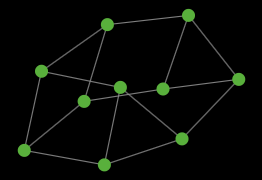
\includegraphics[width=0.8\linewidth]{../Figures/financialContagion1.png}
  \caption{\label{fig:fincont1} Initial graph with 10 agents.}
\end{subfigure}
\quad
\begin{subfigure}{.46\textwidth}
  \centering
  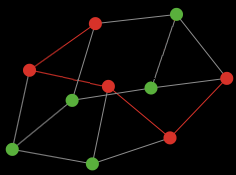
\includegraphics[width=0.8\linewidth]{../Figures/financialContagion2.png}
  \caption{\label{fig:fincont2} Insured agents (red) forms a network}
\end{subfigure}
\caption{\label{fig:fincont} shows how insured agents connects with each other to form a network to achieve super-critical payoffs.}
\end{figure}



